\documentclass{ctexart}
\usepackage{amsmath, amsfonts, amssymb} % 数学公式、符号
\usepackage[colorlinks,linkcolor=red,anchorcolor=blue,citecolor=green]{hyperref}
\usepackage[left=2.50cm, right=2.50cm, top=1.50cm, bottom=1.50cm]{geometry} %页边距
\usepackage{graphicx}   % 图片
\usepackage{multicol}
\usepackage{bm}
\usepackage{listings}
\usepackage{xcolor}
\usepackage{tikz}
\usetikzlibrary{arrows,shapes,chains}
\usepackage{multirow}
\usepackage{algorithm}  
\usepackage{algpseudocode}  
\usepackage{caption}
\floatname{algorithm}{算法}
\renewcommand{\algorithmicrequire}{\textbf{输入:}}  % Use Input in the format of Algorithm  
\renewcommand{\algorithmicensure}{\textbf{输出:}} % Use Output in the format of Algorithm
\usepackage{fancyhdr} %设置页眉、页脚
\pagestyle{fancy}
% 用来设置代码的样式
\lstset{
	basicstyle          =   \sffamily,          % 基本代码风格
	keywordstyle        =   \bfseries,          % 关键字风格
	commentstyle        =   \rmfamily\itshape,  % 注释的风格,斜体
	stringstyle         =   \ttfamily,  % 字符串风格
	flexiblecolumns,                % 别问为什么,加上这个
	numbers             =   left,   % 行号的位置在左边
	showspaces          =   false,  % 是否显示空格,显示了有点乱,所以不现实了
	numberstyle         =   \zihao{-5}\ttfamily,    % 行号的样式,小五号,tt等宽字体
	showstringspaces    =   false,
	captionpos          =   t,      % 这段代码的名字所呈现的位置,t指的是top上面
	frame               =   lrtb,   % 显示边框
}

\lstdefinestyle{Python}{
	language        =   Python, % 语言选Python
	basicstyle      =   \zihao{-5}\ttfamily,
	numberstyle     =   \zihao{-5}\ttfamily,
	keywordstyle    =   \color{blue},
	keywordstyle    =   [2] \color{teal},
	stringstyle     =   \color{magenta},
	commentstyle    =   \color{red}\ttfamily,
	breaklines      =   true,   % 自动换行,建议不要写太长的行
	columns         =   fixed,  % 如果不加这一句,字间距就不固定,很丑,必须加
	basewidth       =   0.5em,
}

\title{\textbf{机器学习实验报告\\{\Large{神经网络}}}} % 标题与子标题
\author{\sffamily{朱天泽}} % 作者
\date{(日期:\today)} % 日期
\vspace{0.7cm}
\setlength{\abovecaptionskip}{0.3cm}   %调整图片标题与图距离
\captionsetup{font={small}}
\setlength{\belowcaptionskip}{0.5cm}   %调整图片标题与下文距离
\begin{document}
	\maketitle
	% 摘要开始
	\noindent{\bf{摘要}}
	在《机器学习》第5章中,我学习了神经网络。在此次实验中,我实现了标准BP算法和累积BP算法,在西瓜数据集3.0上分别用这两个算法训练了一个单隐层网络,并进行了比较。
	
	\noindent{\bf{关键词}} 神经网络;BP算法;分类
	
	% 正文开始
	\section{习题1}
	\subsection{题目理解}
	题目要求:编程实现标准BP算法,在西瓜数据集3.0上训练一个单隐层网络,并做数据分析和结果评价。
	\subsection{标准BP算法原理阐述}
	给定训练集 $D=\{(\bm{x}_1,\bm{y}_i),(\bm{x}_2,\bm{y}_2),\cdots,(\bm{x}_m,\bm{y}_m)\}$,$\bm{x}_i\in\mathbb{R}^d$,$\bm{y}_i\in\mathbb{R}^l$。
	
	\begin{figure}[!htb]
		\centering
		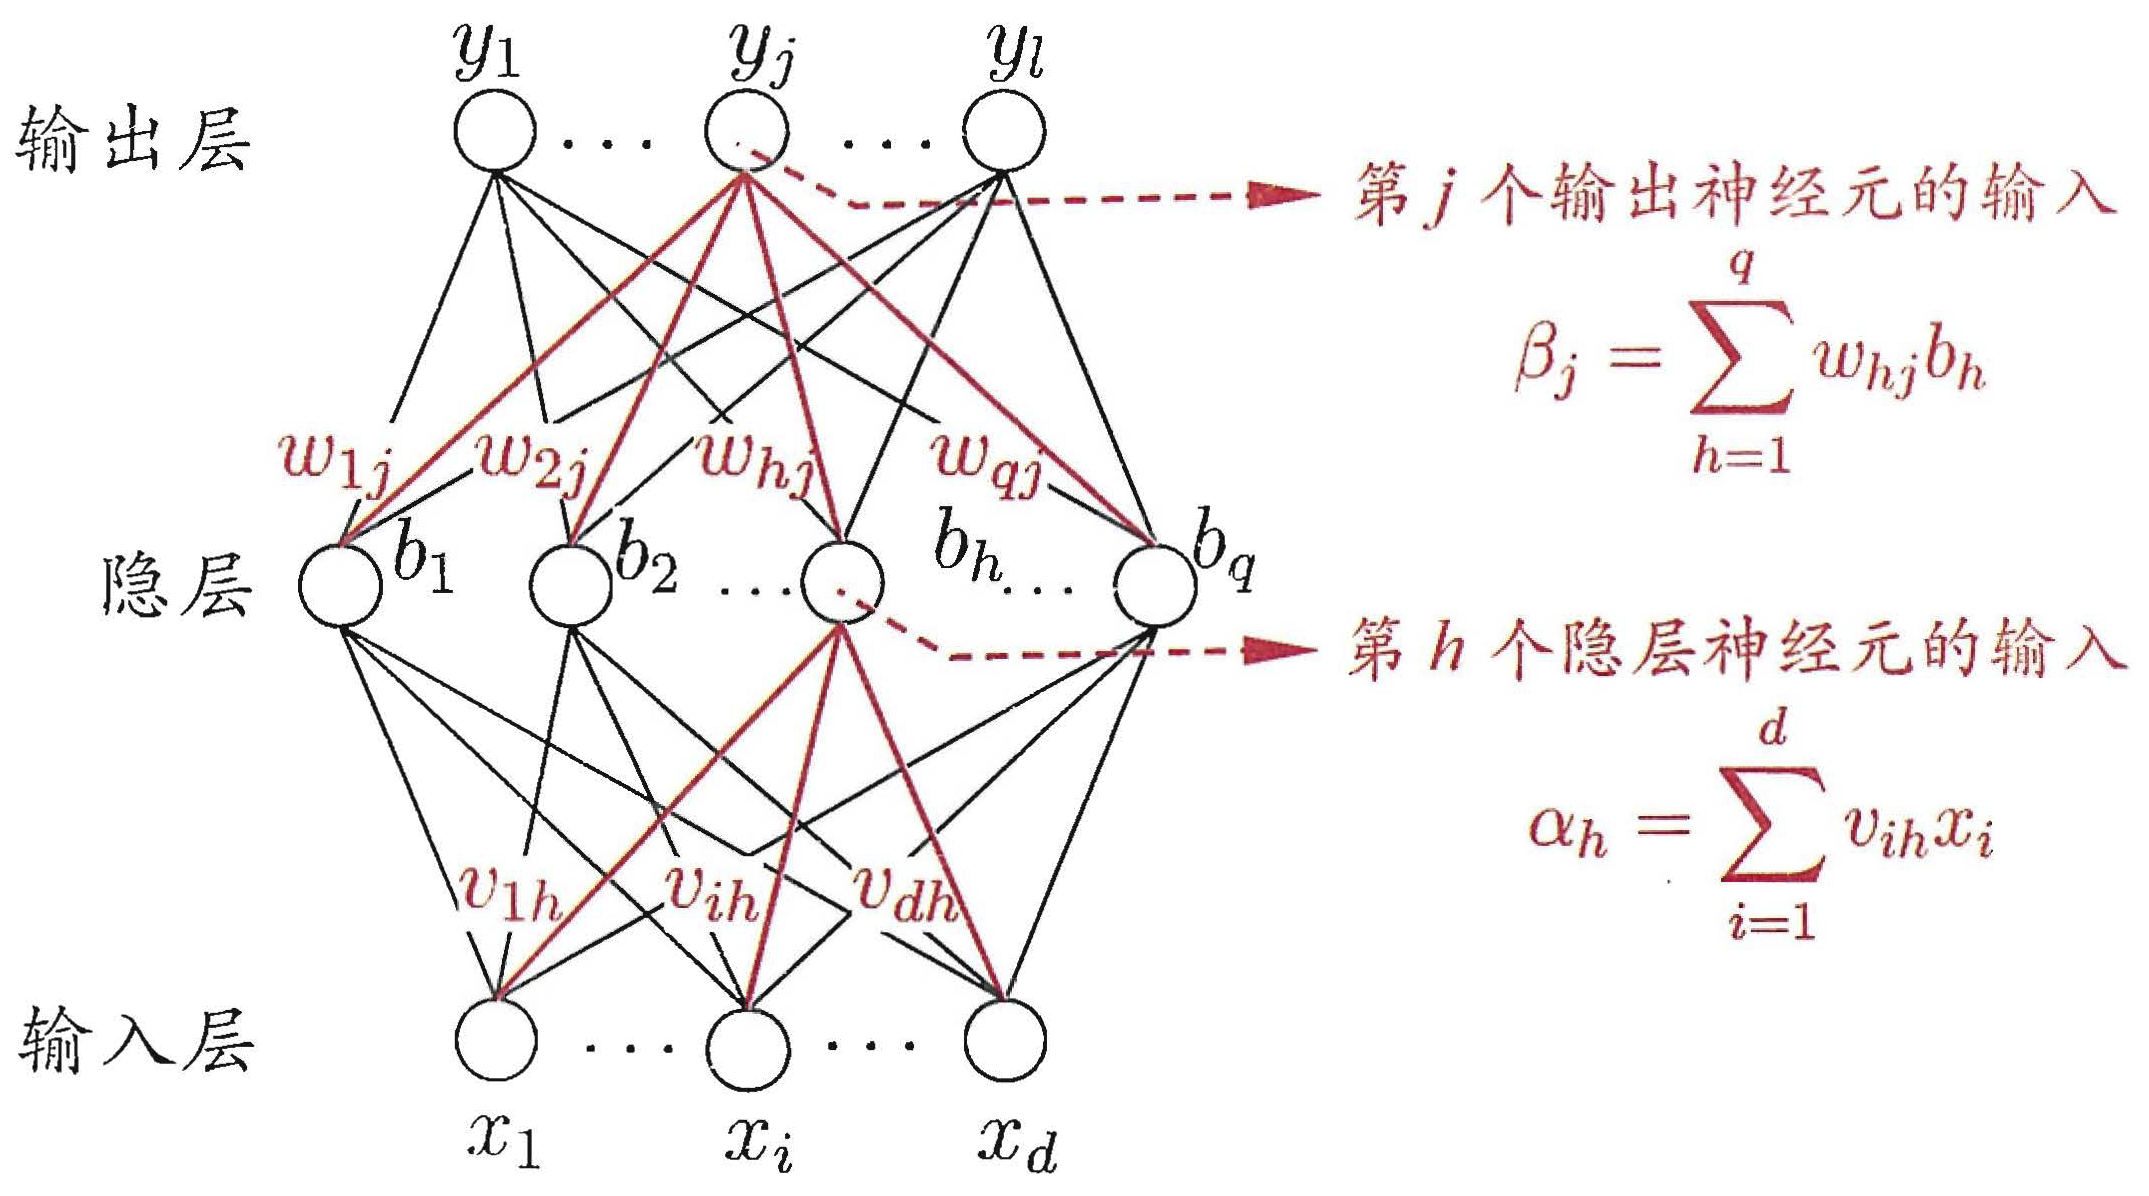
\includegraphics[scale=1,height=6cm]{../image/BP网络及算法中的变量符号.png}
		\caption{BP网络及算法中的变量符号}
		\label{BP网络及算法中的变量符号}
	\end{figure}
	
	为便于讨论,图\ref{BP网络及算法中的变量符号}给出了拥有 $d$ 个输入神经元、$l$ 个输出神经元、$q$ 个隐层网络的多层前馈网络结构,其中输出层第 $j$ 个神经元的阈值用 $\theta_j$ 表示,隐层第 $h$ 个神经元的阈值用 $\gamma_h$ 表示。输入层第 $i$ 个神经元与隐层第 $h$ 个神经元之间的连接权为 $v_{ih}$,隐层第 $h$ 个神经元与输出层第 $j$ 个神经元之间的连接权为 $w_{hj}$。记隐层第 $h$ 个神经元接收到的输入为 $\alpha_h=\sum\limits_{i=1}^d v_{ih}x_i$,输出层第 $j$ 个神经元接收到的输入为 $\beta_j=\sum\limits_{h=1}^q w_{hj}b_h$,其中 $b_h$ 为隐层第 $h$ 个神经元的输出。这里假设隐层和输出层神经元都使用Sigmoid函数 $f(z)=\frac{1}{1+e^{-z}}$。

	对训练样本 $(\bm{x}_k,\bm{y}_k)$,假定神经网络的输出为 $\hat{\bm{y}}_k=(\hat{y}_1^k,\hat{y}_2^k,\cdots,\hat{y}_l^k)$,即
	
	\begin{equation}
		\hat{y}_j^k=f(\beta_j-\theta_j)
		\label{输出标记定义}
	\end{equation}
	
	进一步可定义网络在 $(\bm{x}_k,\bm{y}_k)$ 上的均方误差为
	
	\begin{equation}
		E_{k}=\frac{1}{2} \sum_{j=1}^{l}\left(\hat{y}_{j}^{k}-y_{j}^{k}\right)^{2}
		\label{均方误差式}
	\end{equation}
	
	BP是一个迭代学习算法,在迭代的每一轮中采用广义的感知机学习桂策对参数进行更新估计,任意参数 $\chi$的更新估计式为
	
	\begin{equation}
		\chi\leftarrow\chi+\Delta\chi
		\label{w增量}
	\end{equation}
	
	BP算法基于梯度下降策略,以目标的负梯度方向对参数进行调整。对式\eqref{均方误差式}的误差 $E_k$,给定学习率 $\eta$,有
	
	\begin{equation}
		\Delta w_{h j}=-\eta \frac{\partial E_{k}}{\partial w_{h j}}
	\end{equation}

	注意到 $w_{hj}$ 先影响到第 $j$ 个输出层神经元的输入值 $\beta_j=\sum\limits_{h=1}^q w_{hj}b_h$,再影响到其输出值 $\hat{y}_j^k=f(\beta_j-\theta_j)$,然后影响到 $E_{k}=\frac{1}{2} \sum\limits_{j=1}^{l}\left(\hat{y}_{j}^{k}-y_{j}^{k}\right)^{2}$;根据链式法则,有
	
	\begin{equation}
		\frac{\partial E_{k}}{\partial w_{h j}}=\frac{\partial E_{k}}{\partial \hat{y}_{j}^{k}} \cdot \frac{\partial \hat{y}_{j}^{k}}{\partial \beta_{j}} \cdot \frac{\partial \beta_{j}}{\partial w_{h j}}
		\label{链式偏导}
	\end{equation}

	根据 $\beta_{j}$ 的定义,显然有
	
	\begin{equation}
		\frac{\partial \beta_{j}}{\partial w_{h j}}=b_{h}
		\label{bh}
	\end{equation}

	基于Sigmoid函数良好的性质 $f'(x)=f(x)(1-f(x))$,根据式\eqref{输出标记定义}和式\eqref{均方误差式},有
	
	\begin{equation}
		\begin{aligned}
			g_{j} &=-\frac{\partial E_{k}}{\partial \hat{y}_{j}^{k}} \cdot \frac{\partial \hat{y}_{j}^{k}}{\partial \beta_{j}} \\
			&=-\left(\hat{y}_{j}^{k}-y_{j}^{k}\right) f^{\prime}\left(\beta_{j}-\theta_{j}\right) \\
			&=\hat{y}_{j}^{k}\left(1-\hat{y}_{j}^{k}\right)\left(y_{j}^{k}-\hat{y}_{j}^{k}\right)
		\end{aligned}
		\label{gj}
	\end{equation}

	将式\eqref{bh}和式\eqref{gj}代入式\eqref{链式偏导},再代入式\eqref{w增量},得到BP算法中关于 $w_{hj}$ 的更新公式
	
	\begin{equation}
		\Delta w_{h j}=\eta g_{j} b_{h}
	\end{equation}

	类似可得
	
	\begin{equation}
		\begin{aligned}
			\frac{\partial E_{k}}{\partial \theta_{j}} &=\frac{\partial E_{k}}{\partial \hat{y}_{j}^{k}} \cdot \frac{\partial \hat{y}_{j}^{k}}{\partial \theta_{j}} \\
			&=\frac{\partial E_{k}}{\partial \hat{y}_{j}^{k}} \cdot \frac{\partial\left[f\left(\beta_{j}-\theta_{j}\right)\right]}{\partial \theta_{j}} \\
			&=-\frac{\partial E_{k}}{\partial \hat{y}_{j}^{k}} \cdot f^{\prime}\left(\beta_{j}-\theta_{j}\right)\\
			&=\left(y_{j}^{k}-\hat{y}_{j}^{k}\right) \hat{y}_{j}^{k}\left(1-\hat{y}_{j}^{k}\right) \\
		\end{aligned}
	\end{equation}

	\begin{equation}
		\begin{aligned}
			\frac{\partial E_{k}}{\partial v_{i h}} &=\sum_{j=1}^{l} \frac{\partial E_{k}}{\partial \hat{y}_{j}^{k}} \cdot \frac{\partial \hat{y}_{j}^{k}}{\partial \beta_{j}} \cdot \frac{\partial \beta_{j}}{\partial b_{h}} \cdot \frac{\partial b_{h}}{\partial \alpha_{h}} \cdot \frac{\partial \alpha_{h}}{\partial v_{i h}} \\
			&=\sum_{j=1}^{l} \frac{\partial E_{k}}{\partial \hat{y}_{j}^{k}} \cdot \frac{\partial \hat{y}_{j}^{k}}{\partial \beta_{j}} \cdot \frac{\partial \beta_{j}}{\partial b_{h}} \cdot \frac{\partial b_{h}}{\partial \alpha_{h}} \cdot x_{i} \\
			&=\sum_{j=1}^{l} \frac{\partial E_{k}}{\partial \hat{y}_{j}^{k}} \cdot \frac{\partial \hat{y}_{j}^{k}}{\partial \beta_{j}} \cdot \frac{\partial \beta_{j}}{\partial b_{h}} \cdot f^{\prime}\left(\alpha_{h}-\gamma_{h}\right) \cdot x_{i} \\
			&=\sum_{j=1}^{l} \frac{\partial E_{k}}{\partial \hat{y}_{j}^{k}} \cdot \frac{\partial \hat{y}_{j}^{k}}{\partial \beta_{j}} \cdot w_{h j} \cdot f^{\prime}\left(\alpha_{h}-\gamma_{h}\right) \cdot x_{i} \\
			&=\sum_{j=1}^{l}\left(-g_{j}\right) \cdot w_{h j} \cdot f^{\prime}\left(\alpha_{h}-\gamma_{h}\right) \cdot x_{i} \\
			&=-f^{\prime}\left(\alpha_{h}-\gamma_{h}\right) \cdot \sum_{j=1}^{l} g_{j} \cdot w_{h j} \cdot x_{i} \\
			&=-b_{h}\left(1-b_{h}\right) \cdot \sum_{j=1}^{l} g_{j} \cdot w_{h j} \cdot x_{i} \\
		\end{aligned}
	\end{equation}

	\begin{equation}
		\begin{aligned}
			\frac{\partial E_{k}}{\partial \gamma_{h}} &=\sum_{j=1}^{l} \frac{\partial E_{k}}{\partial \hat{y}_{j}^{k}} \cdot \frac{\partial \hat{y}_{j}^{k}}{\partial \beta_{j}} \cdot \frac{\partial \beta_{j}}{\partial b_{h}} \cdot \frac{\partial b_{h}}{\partial \gamma_{h}} \\
			&=-\sum_{j=1}^{l} \frac{\partial E_{k}}{\partial \hat{y}_{j}^{k}} \cdot \frac{\partial \hat{y}_{j}^{k}}{\partial \beta_{j}} \cdot \frac{\partial \beta_{j}}{\partial b_{h}} \cdot f^{\prime}\left(\alpha_{h}-\gamma_{h}\right)\\
			&=-\sum_{j=1}^{l} \frac{\partial E_{k}}{\partial \hat{y}_{j}^{k}} \cdot \frac{\partial \hat{y}_{j}^{k}}{\partial \beta_{j}} \cdot w_{h j} \cdot f^{\prime}\left(\alpha_{h}-\gamma_{h}\right) \\
			&=-\sum_{j=1}^{l} \frac{\partial E_{k}}{\partial \hat{y}_{j}^{k}} \cdot \frac{\partial \hat{y}_{j}^{k}}{\partial \beta_{j}} \cdot w_{h j} \cdot b_{h}\left(1-b_{h}\right) \\
			&=\sum_{j=1}^{l} g_{j} \cdot w_{h j} \cdot b_{h}\left(1-b_{h}\right) \\
		\end{aligned}
	\end{equation}

	令
	
	\begin{equation}
		e_h=b_{h}\left(1-b_{h}\right) \sum_{j=1}^{l} w_{h j} g_{j}
	\end{equation}

	进一步得到其余变量的增量
	
	\begin{equation}
		\Delta\theta_{j}=-\eta g_j
	\end{equation}
	
	\begin{equation}
		\Delta v_{ih}=\eta e_h x_i
	\end{equation}

	\begin{equation}
		\Delta \gamma_h=-\eta e_h
	\end{equation}
	
	\subsection{标准BP算法设计思路}
	将上述推导进一步写成矩阵形式,定义
	
	\begin{equation}
		\bm{g}=\begin{bmatrix}
			g_1\\g_2\\\vdots\\g_l
		\end{bmatrix}\quad
		\bm{e}=\begin{bmatrix}
			e_1\\e_2\\\vdots\\e_q
		\end{bmatrix}\quad
	\end{equation}

	\begin{equation}
		\bm{x}=\begin{bmatrix}
			x_1\\x_2\\\vdots\\x_d
		\end{bmatrix}\quad
		\bm{y}=\begin{bmatrix}
			y_1\\y_2\\\vdots\\y_l
		\end{bmatrix}\quad
		\bm{\alpha}=\begin{bmatrix}
			\alpha_1\\\alpha_2\\\vdots\\\alpha_q
		\end{bmatrix}\quad
		\bm{b}=\begin{bmatrix}
			b_1\\b_2\\\vdots\\b_q
		\end{bmatrix}\quad
		\bm{\beta}=\begin{bmatrix}
			\beta_1\\\beta_2\\\vdots\\\beta_l
		\end{bmatrix}\quad
		\hat{\bm{y}}=\begin{bmatrix}
			\hat{y}_1\\\hat{y}_2\\\vdots\\\hat{y}_l
		\end{bmatrix}
	\end{equation}
	
	\begin{equation}
		\bm{\theta}=\begin{bmatrix}
			\theta_1\\\theta_2\\\vdots\\\theta_l
		\end{bmatrix}\quad
		\bm{\gamma}=\begin{bmatrix}
			\gamma_1\\\gamma_2\\\vdots\\\gamma_q
		\end{bmatrix}\quad
		\bm{V}=\begin{bmatrix}  
			v_{11} & v_{12} & \cdots & v_{1q} \\  
			v_{21} & v_{22} & \cdots & v_{2q} \\  
			\vdots & \vdots & \ddots & \vdots \\  
			v_{d1} & v_{d2} & \cdots & v_{dq}  
		\end{bmatrix}\quad
		\bm{W}=\begin{bmatrix}  
			w_{11} & w_{12} & \cdots & w_{1l} \\  
			w_{21} & w_{22} & \cdots & w_{2l} \\  
			\vdots & \vdots & \ddots & \vdots \\  
			w_{q1} & w_{q2} & \cdots & w_{ql}
		\end{bmatrix}
	\end{equation}
	
	易得
	
	\begin{equation}
		\bm{g}=\hat{\bm{y}}\circ (\bm{I}-\hat{\bm{y}})\circ(\bm{y}-\hat{\bm{y}})
	\end{equation}
	
	\begin{equation}
		\bm{e}=\bm{b}\circ(\bm{I}-\bm{b})\circ(\bm{W}\times \bm{g})
	\end{equation}
	
	\begin{equation}
		\bm{\alpha}=\bm{V}^\mathrm{T}\bm{x}
	\end{equation}

	\begin{equation}
		\bm{\beta}=\bm{W}^\mathrm{T}\bm{b}
	\end{equation}

	进一步可得
	
	\begin{equation}
		\Delta\bm{W}=\eta\bm{b}\bm{g}^\mathrm{T}
	\end{equation}
	
	\begin{equation}
		\Delta\bm{\theta}=-\eta\bm{g}
	\end{equation}

	\begin{equation}
		\Delta\bm{V}=\eta\bm{x}\bm{e}^\mathrm{T}
	\end{equation}

	\begin{equation}
		\Delta\bm{\gamma}=-\eta\bm{e}
	\end{equation}

	综上所述,将参数包装为向量和矩阵,参数之间的运算都为Hadamard积或矩阵乘法,在NumPy中可用运算符“*”计算Hadamard积、用函数“dot”或运算符“@”计算矩阵乘法。
	
	\begin{figure}[!htb]
		\centering
		\scriptsize  
		% 流程图定义基本形状
		\tikzstyle{startstop} = [rectangle, rounded corners, minimum width = 2cm, minimum height=0.5cm,text centered, draw = black]
		\tikzstyle{io} = [trapezium, trapezium left angle=70, trapezium right angle=110, minimum width=1cm, minimum height=0.6cm, text centered, draw=black]
		\tikzstyle{process} = [rectangle, minimum width=3cm, minimum height=0.6cm, text centered, draw=black]
		\tikzstyle{decision} = [diamond, aspect = 3, text centered, draw=black]
		\tikzstyle{point}=[coordinate,on grid] 
		% 箭头形式
		\tikzstyle{arrow} = [->,>=stealth]
		\begin{tikzpicture}
			\node[startstop](start){ 开始};
			\node[io,below=of start](define){ 输入数据集};
			\node[process,right=of define](init){ 初始化参数 $w_{hj},\theta_j,v_{ih},\gamma_h,\eta$};
			\node[process,right=of init](error){ 计算误差项 $E=\frac{1}{m}\sum\limits_{k=1}^m ||\hat{\bm{y}}_k-\bm{y}_k||_2^2$};
			\node[decision,below=of error](decision){ 与上一次迭代误差变化 $\Delta E\leqslant\varepsilon$};
			\node[process,below=of decision](for){ \textbf{for all} $(\bm{x}_k,\bm{y}_k)\in D$};
			\node[io,left=of decision] (输出) { 输出$w_{hj},\theta_j,v_{ih},\gamma_h$};
			\node[startstop,left=of 输出] (stop) { 结束};
			\node[process,left=of for](输出值){ 计算当前样本的输出 $\hat{\bm{y}}_k$};
			\node[process,below=of 输出值](中间值){ 计算中间值 $\bm{e},\bm{g}$};
			\node[process,left=of 中间值](增量){ 计算增量 $\Delta \bm{W},\Delta\bm{\theta},\Delta \bm{v},\Delta\bm{\gamma}$};
			\node[process,above=of 增量](cal){ 更新参数 $\bm{W},\bm{\theta},\bm{V},\bm{\gamma}$};
			\node[point,right of=for,node distance=4.4cm](point1){};
			\draw[arrow](define)--(init);
			\draw[arrow](init)--(error);
			\draw[arrow] (decision)-- node[right]{否}(for);
			\draw[arrow] (输出值)--(中间值);
			\draw[arrow] (decision)-- node[above]{是}(输出);
			\draw[arrow](error)--(decision);
			\draw[arrow](中间值)--(增量);
			\draw[arrow](增量)--(cal);
			\draw[arrow](输出)--(stop);
			\draw[arrow](start)--(define);
			\draw[arrow](for)--(输出值);
			\draw[-](for.east)--(point1);
			\draw[arrow](point1)|-(error.east);
		\end{tikzpicture}
		\caption{标准BP算法流程}
		\label{标准BP算法流程}
	\end{figure}

	标准BP算法的流程如图\ref{标准BP算法流程},对每个训练样本,BP算法执行以下操作:先将输入示例提供给输入神经元,信号将逐层前传,直到产生输出层的结果;然后计算输出层的误差,再将误差逆向传播至隐层神经元;最后根据隐层神经元的误差来对连接权和阈值进行调整。该迭代过程循环进行,直到达到设置的停止条件位置。
	
	在实验中,我们使用西瓜数据集3.0训练单隐层神经网络。在西瓜数据集3.0中,“色泽”“根蒂”“敲声”“纹理”“脐部”“触感”为离散值,而“密度”、“含糖率”为连续值;我们需要将离散值映射为连续值来方便计算;举例来说,色泽有三种取值,分别为“青绿”“乌黑”“浅白”,可对三个取值分别赋值为1、2、3;此外,还需要将结果是否为好瓜映射为0、1的布尔值。

	\subsection{核心代码分析}
	
	标准BP算法的核心代码如下。代码中用数组errors记录了每一次迭代的误差项。标准BP算法遍历每一个样本,每个样本都对参数值进行更新。\\
	
	\lstinputlisting[style=Python]{../code/core/BP.txt}
	
	\subsection{实验结果分析}
	
	在本次实验中,我利用西瓜数据集3.0,用标准BP算法训练了一个单隐层网络。
	
	在标准BP算法中,参数 $\bm{W}$、$\bm{V}$、$\bm{\theta}$、$\bm{\gamma}$ 通过迭代得到,不同的训练样本集合 $\{(\bm{x}_k,\bm{y}_k)\}_{k=1}^m$ 会得到不同的参数值。不同于神经网络中的参数,学习率 $\eta$ 是一个超参数,实际上指征了每一步迭代时向梯度负方向前进的速率。
	
	参数 $\bm{W}$、$\bm{V}$、$\bm{\theta}$、$\bm{\gamma}$ 均随机初始化,而 $\eta$ 可根据具体问题指定适合的值。在实验中,我随机初始化了4组参数,并对每一组参数取不同的 $\eta$ 训练神经网络,得到其收敛速率。
	结合图\ref{标准1}、图\ref{标准2}、图\ref{标准3}、图\ref{标准4},大约在前50次迭代,不论 $\eta$ 值如何,总体均方误差均快速下降;随后,$\eta$ 越大,收敛速度越快。$\eta$ 并不是越大越好,可以发现当 $\eta$ 较大时,曲线的抖动会更为剧烈,这可能是在极小值点附近跳跃造成的;但是这种抖动也可能带来意外收益,即跳出局部最优解,到达更优的情况,这就解释了当 $\eta$ 较大时,会在一段时间的迭代后,均方误差再次快速下降的现象。
	
	\begin{figure}[!htb]
		\centering
		\begin{minipage}{0.49\linewidth}
			\centering
			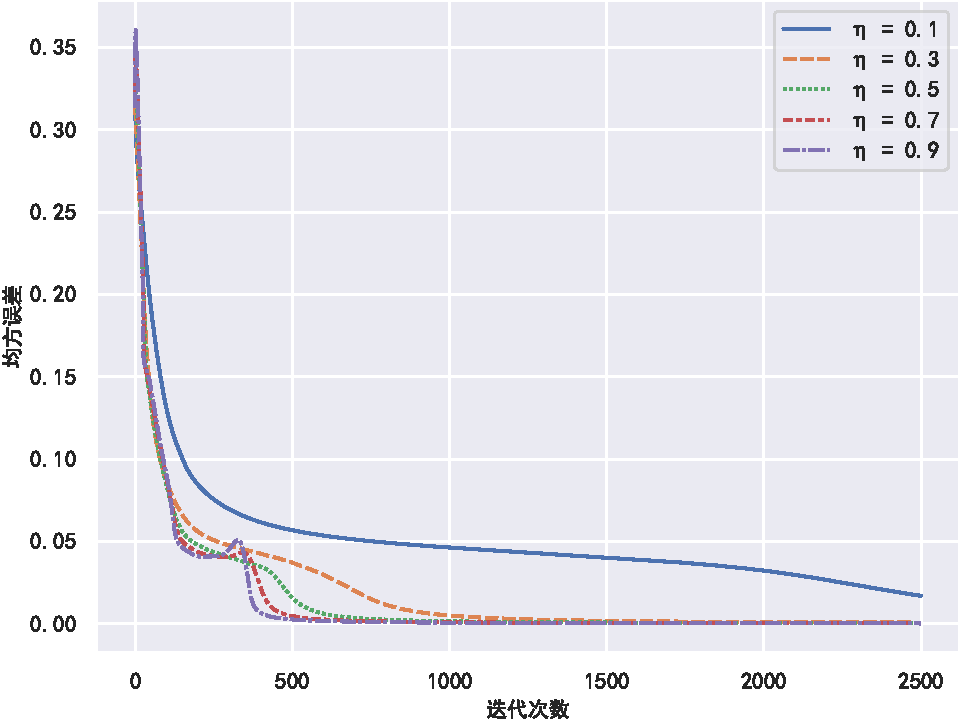
\includegraphics[width=\textwidth]{../image/标准BP抖动1.pdf}
			\caption{标准BP算法取不同$\eta$ 时的迭代速度(1)}
			\label{标准1}%文中引用该图片代号
		\end{minipage}
		\begin{minipage}{0.49\linewidth}
			\centering
			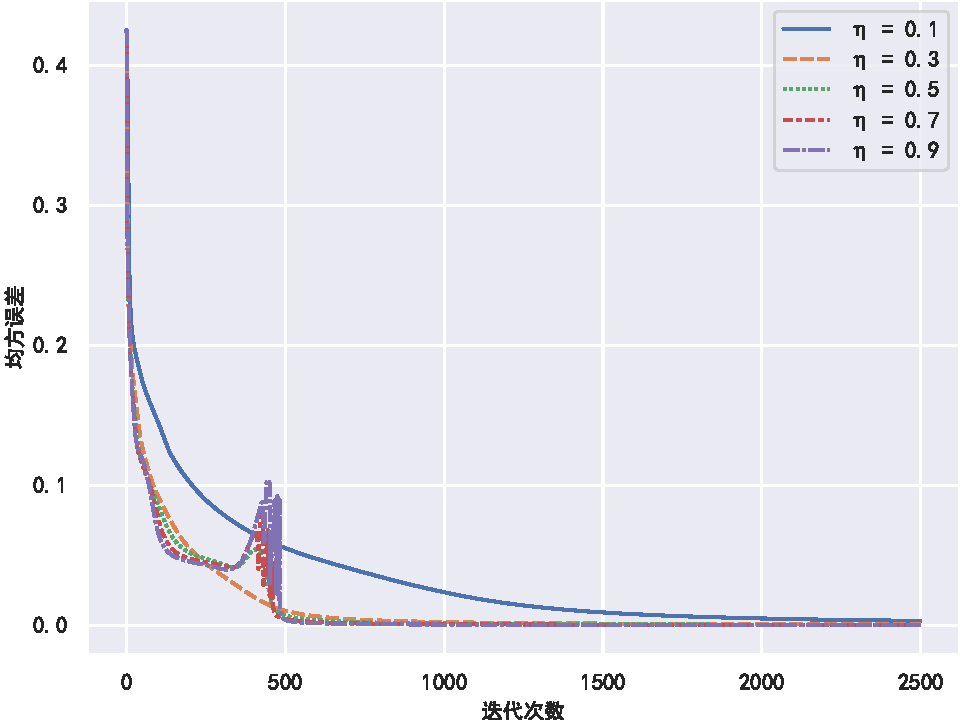
\includegraphics[width=\textwidth]{../image/标准BP抖动2.pdf}
			\caption{标准BP算法取不同$\eta$ 时的迭代速度(2)}
			\label{标准2}%文中引用该图片代号
		\end{minipage}
		%让图片换行,
		
		\begin{minipage}{0.49\linewidth}
			\centering
			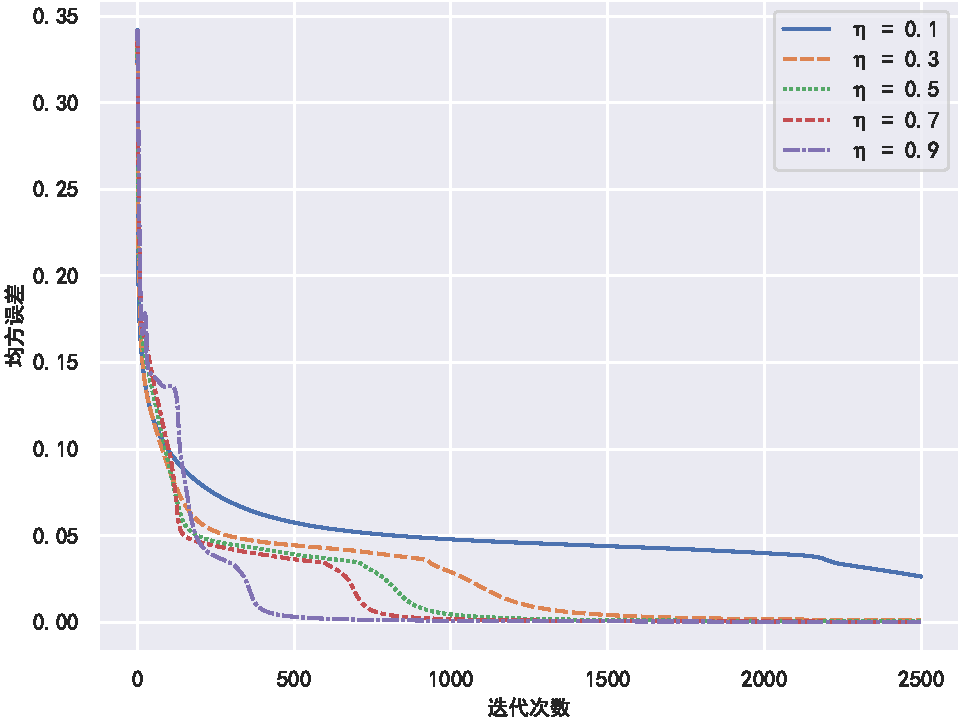
\includegraphics[width=\textwidth]{../image/标准BP抖动3.pdf}
			\caption{标准BP算法取不同$\eta$ 时的迭代速度(3)}
			\label{标准3}%文中引用该图片代号
		\end{minipage}
		\begin{minipage}{0.49\linewidth}
			\centering
			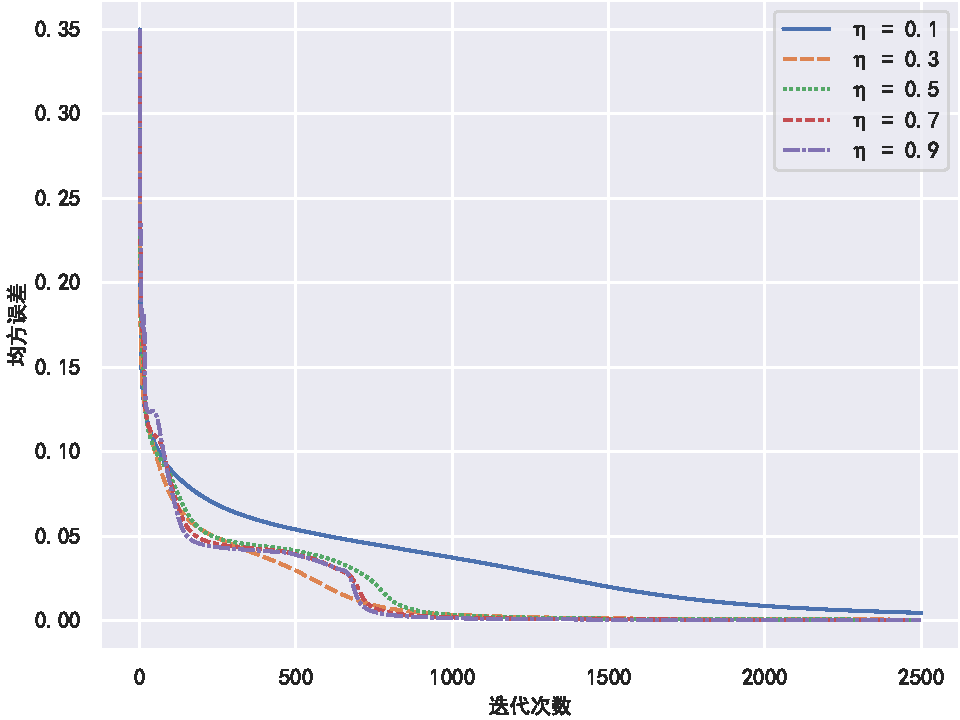
\includegraphics[width=\textwidth]{../image/标准BP抖动4.pdf}
			\caption{标准BP算法取不同$\eta$ 时的迭代速度(4)}
			\label{标准4}%文中引用该图片代号
		\end{minipage}
	\end{figure}

	\begin{figure}[!htb]
		\centering
		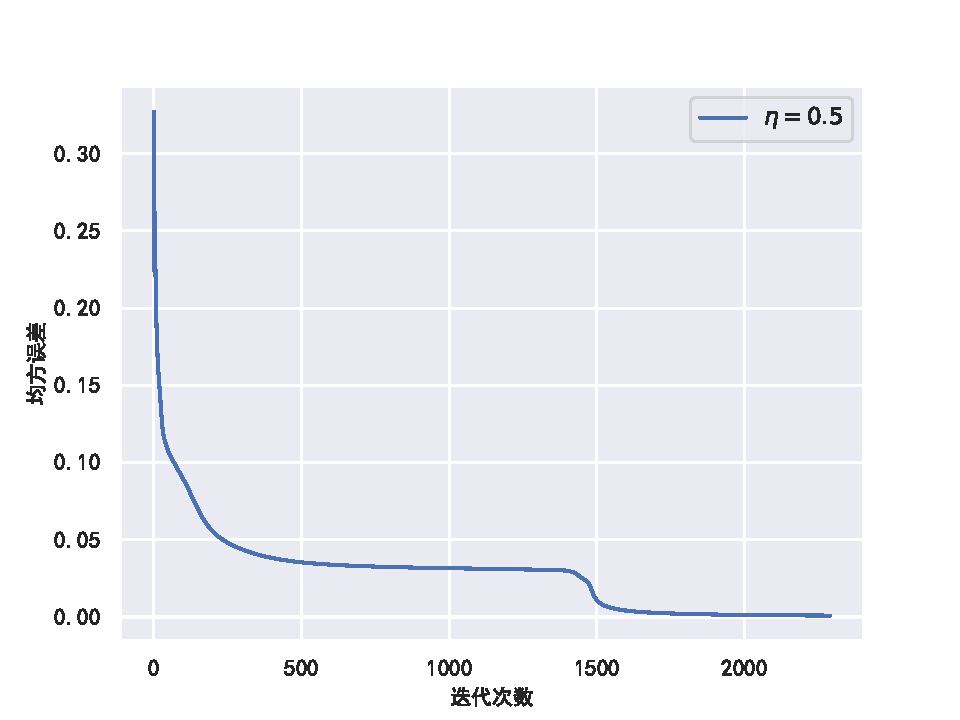
\includegraphics[height=7cm]{../image/标准BP较好值.pdf}
		\caption{标准BP算法超参数 $\eta$ 在西瓜数据集3.0上的适宜值}
		\label{标准BP适宜值}
	\end{figure}

	总结得出,对于西瓜数据集3.0来说,$\eta=0.5$ 是较为适宜的值;如图 \ref{标准BP适宜值},当 $\eta=0.5$ 时,曲线跳跃区间较小,收敛速度也比较快,且与学习率更大时的均方误差收敛值相差不大。
	
	\subsection{学习收获}
	
	在此次实验中,我实现了标准BP算法,并对学习率参数 $\eta$ 进行了一些研究,得到了迭代收敛速率关于学习率的一些性质。
	
	在实际中,很难使用一个确定的值为最佳的学习率。在误差变化平坦区内,我们希望学习率增大的,因为太小会使得训练次数增加,增大会加速脱离平坦区。在误差变化很大的区域,太大会容易跨过较窄的最低点,这个最低点可能是全局最优点,同时会产生振荡,反而是迭代次数增加。因此为了加速收敛,一个较好的解决思路就是让学习率根据具体情况进行动态调整。查阅资料可知,有AdaGrad、Adadelta、RMSProp、Adam等方法来动态调整学习率。
	
	还有一些内容并未在实验中涉及,未来可进一步研究隐层维度、参数初始化方式等因素对算法的影响。
	
	\subsection{参考资料}
	
	\begin{itemize}
		\item 《机器学习》5.3;周志华;清华大学出版社。
		\item 《机器学习公式详解》5.12,5.13,5.14,5.15;谢文睿,秦州;人民邮电出版社。
		\item \href{https://blog.csdn.net/weixin_42398658/article/details/83958133}{深度学习 --- BP算法详解(BP算法的优化)}
	\end{itemize}

	\section{习题2}
	
	\subsection{题目理解}
	
	题目要求:编程实现累积BP算法,在西瓜数据集3.0上训练一个单隐层网络,做数据分析和结果评价,并和标准BP算法进行比较。
	
	\subsection{累积BP算法原理阐述}
	
	需要注意的是,BP算法的目标是要最小化训练集 $D$ 上的累积误差
	
	\begin{equation}
		E=\frac{1}{m}\sum_{k=1}^m E_k
	\end{equation}

	上面介绍的“标准BP算法”每次仅针对一个训练样例更新连接权和阈值,也就是说,“标准BP算法”的更新规则是基于单个的 $E_k$ 推导而得,如果类似地推导出基于累积误差最小化的更新规则,就得到了“累积BP算法”。
	
	对于神经网络中任意结点上的一个参数 $\chi$
	
	\begin{equation}
		\frac{\partial E}{\partial \chi}=\frac{1}{m}\sum_{k=1}^{m}\frac{\partial E_k}{\partial \chi}
	\end{equation}

	给定学习率 $\eta$,有
	
	\begin{equation}
		\Delta \chi=\frac{1}{m}\sum_{k=1}^{m}\left(-\eta\frac{\partial E_k}{\partial \chi}\right)
		\label{累积BP更新式}
	\end{equation}
	
	式\eqref{累积BP更新式}中的 $\left(-\eta\frac{\partial E_k}{\partial \chi}\right)$一项,实际上就是标准BP算法中每个参数每一步迭代的增量;累积BP算法直接针对累积误差最小化,参数增量为每一个样本求得增量的平均值。
	
	\subsection{累积BP算法设计思路}
	
	仿照标准BP算法的思路,我们可以将推导写成矩阵形式方便程序处理;由于累积BP算法在读取整个训练集 $D$ 一遍后才对参数进行更新,我们不妨将所有样本及每个样本在迭代时产生的向量 $\bm{g}$ 和 $\bm{e}$ 组合成矩阵
	
	\begin{equation}
		\bm{G}=\begin{bmatrix}
			\bm{g}_1\\\bm{g}_2\\\vdots\\\bm{g}_m
		\end{bmatrix}\quad
		\bm{E}=\begin{bmatrix}
			\bm{e}_1\\\bm{e}_2\\\vdots\\\bm{e}_m
		\end{bmatrix}\quad
	\end{equation}
		
	\begin{equation}
		\bm{X}=\begin{bmatrix}
			\bm{x}_1^\mathrm{T}\\\bm{x}_2^\mathrm{T}\\\vdots\\\bm{x}_m^\mathrm{T}
		\end{bmatrix}\quad
		\bm{Y}=\begin{bmatrix}
			\bm{y}_1^\mathrm{T}\\\bm{y}_2^\mathrm{T}\\\vdots\\\bm{y}_m^\mathrm{T}
		\end{bmatrix}\quad
		\bm{A}=\begin{bmatrix}
			\bm{\alpha}^\mathrm{T}\\\bm{\alpha}^\mathrm{T}\\\vdots\\\bm{\alpha}_m^\mathrm{T}
		\end{bmatrix}\quad
		\bm{B}=\begin{bmatrix}
			\bm{b}_1^\mathrm{T}\\\bm{b}_2^\mathrm{T}\\\vdots\\\bm{b}_m^\mathrm{T}
		\end{bmatrix}\quad
		\bm{\varXi}=\begin{bmatrix}
			\bm{\beta}_1^\mathrm{T}\\\bm{\beta}_2^\mathrm{T}\\\vdots\\\bm{\beta}_m^\mathrm{T}
		\end{bmatrix}\quad
		\hat{\bm{Y}}=\begin{bmatrix}
			\hat{\bm{y}}_1^\mathrm{T}\\\hat{\bm{y}}_2^\mathrm{T}\\\vdots\\\hat{\bm{y}}_m^\mathrm{T}
		\end{bmatrix}
	\end{equation}

	\begin{equation}
		\bm{\theta}=\begin{bmatrix}
			\theta_1\\\theta_2\\\vdots\\\theta_l
		\end{bmatrix}\quad
		\bm{\gamma}=\begin{bmatrix}
			\gamma_1\\\gamma_2\\\vdots\\\gamma_q
		\end{bmatrix}\quad
		\bm{V}=\begin{bmatrix}  
			v_{11} & v_{12} & \cdots & v_{1q} \\  
			v_{21} & v_{22} & \cdots & v_{2q} \\  
			\vdots & \vdots & \ddots & \vdots \\  
			v_{d1} & v_{d2} & \cdots & v_{dq}  
		\end{bmatrix}\quad
		\bm{W}=\begin{bmatrix}  
			w_{11} & w_{12} & \cdots & w_{1l} \\  
			w_{21} & w_{22} & \cdots & w_{2l} \\  
			\vdots & \vdots & \ddots & \vdots \\  
			w_{q1} & w_{q2} & \cdots & w_{ql}
		\end{bmatrix}
	\end{equation}

	易得
	
	\begin{equation}
		\bm{G}=\hat{\bm{Y}}\circ\left(\bm{I}-\hat{\bm{Y}}\right)\circ\left(\bm{Y}-\hat{\bm{Y}}\right)
	\end{equation}
	
	\begin{equation}
		\bm{E}=\bm{B}\circ(\bm{I}-\bm{B})\circ\left(\bm{G}\times\bm{W}^\mathrm{T}\right)
	\end{equation}

	\begin{equation}
		\bm{A}=\bm{X}\bm{V}
	\end{equation}

	\begin{equation}
		\bm{\varXi}=\bm{B}\bm{W}
	\end{equation}

	进一步可得
	
	\begin{equation}
		\Delta\bm{W}=\frac{\eta}{m} \bm{B}^\mathrm{T}\bm{G}
	\end{equation}
	
	\begin{equation}
		\Delta\bm{\theta}=-\frac{\eta}{m}\sum_{k=1}^m \bm{g}_k
	\end{equation}

	\begin{equation}
		\Delta\bm{V}=\frac{\eta}{m}\bm{X}^\mathrm{T}\bm{E}
	\end{equation}

	\begin{equation}
		\Delta\bm{\gamma}=-\frac{\eta}{m}\sum_{k=1}^m \bm{e}_k
	\end{equation}

		综上所述,将参数包装为向量和矩阵,参数之间的运算都为Hadamard积或矩阵乘法,在NumPy中可用运算符“*”计算Hadamard积、用函数“dot”或运算符“@”计算矩阵乘法。
	
	\begin{figure}[!htb]
		\centering
		\scriptsize  
		% 流程图定义基本形状
		\tikzstyle{startstop} = [rectangle, rounded corners, minimum width = 2cm, minimum height=0.5cm,text centered, draw = black]
		\tikzstyle{io} = [trapezium, trapezium left angle=70, trapezium right angle=110, minimum width=1cm, minimum height=0.6cm, text centered, draw=black]
		\tikzstyle{process} = [rectangle, minimum width=3cm, minimum height=0.6cm, text centered, draw=black]
		\tikzstyle{decision} = [diamond, aspect = 3, text centered, draw=black]
		\tikzstyle{point}=[coordinate,on grid] 
		% 箭头形式
		\tikzstyle{arrow} = [->,>=stealth]
		\begin{tikzpicture}
			\node[startstop](start){ 开始};
			\node[io,below=of start](define){ 输入数据集};
			\node[process,right=of define](init){ 初始化参数 $\bm{W},\bm{\theta},\bm{V},\bm{\gamma},\eta$};
			\node[process,right=of init](error){ 计算误差项 $E=\frac{1}{m}\sum\limits_{k=1}^m ||\hat{\bm{y}}_k-\bm{y}_k||_2^2$};
			\node[decision,below=of error](decision){ 与上一次迭代误差变化 $\Delta E\leqslant\varepsilon$};
			\node[io,left=of decision] (输出) { 输出$\bm{W},\bm{\theta},\bm{V},\bm{\gamma}$};
			\node[startstop,left=of 输出] (stop) { 结束};
			\node[process,below=of decision](输出值){ 计算样本的输出 $\hat{\bm{Y}}$};
			\node[process,below=of 输出值](中间值){ 计算中间值 $\bm{E},\bm{G}$};
			\node[process,left=of 中间值](增量){ 计算增量 $\Delta \bm{W},\Delta\bm{\theta},\Delta \bm{V},\Delta\bm{\gamma}$};
			\node[process,above=of 增量](cal){ 更新参数 $\bm{W},\bm{\theta},\bm{V},\bm{\gamma}$};
			\node[point,left of=cal,node distance=2.3cm](point1){};
			\node[point,below of=point1,node distance=2.4cm](point2){};
			\node[point,right of=point2,node distance=10cm](point3){};
			\draw[arrow](define)--(init);
			\draw[arrow](init)--(error);
			\draw[arrow] (decision)-- node[right]{否}(输出值);
			\draw[arrow] (输出值)--(中间值);
			\draw[arrow] (decision)-- node[above]{是}(输出);
			\draw[arrow](error)--(decision);
			\draw[arrow](中间值)--(增量);
			\draw[arrow](增量)--(cal);
			\draw[arrow](输出)--(stop);
			\draw[arrow](start)--(define);
			\draw[-](cal)--(point1);
			\draw[-](point1)--(point2);
			\draw[-](point2)--(point3);
			\draw[arrow](point3)|-(error.east);
		\end{tikzpicture}
		\caption{累积BP算法流程}
		\label{累积BP算法流程}
	\end{figure}
	
	累积BP算法的流程如图\ref{累积BP算法流程},累积BP算法执行以下操作:将输入样本一次性提供给输入神经元,信号将逐层前传,直到产生输出层的结果;然后计算输出层的误差,再将误差逆向传播至隐层神经元;最后根据隐层神经元的误差来对连接权和阈值进行调整。该迭代过程循环进行,直到达到设置的停止条件为止。
	
	在实验中,我们使用西瓜数据集3.0训练单隐层神经网络。在西瓜数据集3.0中,“色泽”“根蒂”“敲声”“纹理”“脐部”“触感”为离散值,而“密度”、“含糖率”为连续值;我们需要将离散值映射为连续值来方便计算;举例来说,色泽有三种取值,分别为“青绿”“乌黑”“浅白”,可对三个取值分别赋值为1、2、3;此外,还需要将结果是否为好瓜映射为0、1的布尔值。
		
	\subsection{核心代码分析}
	
	累积BP算法的核心代码如下。代码中用数组errors记录了每一次迭代的误差项。累积BP算法一次性遍历样本,再对参数值进行更新。\\
	
	\lstinputlisting[style=Python]{../code/core/ABP.txt}
	
	\subsection{实验结果分析}
	
	在本次实验中,我利用西瓜数据集3.0,用标准BP算法训练了一个单隐层网络。
	
	在标准BP算法中,参数 $\bm{W}$、$\bm{V}$、$\bm{\theta}$、$\bm{\gamma}$ 通过迭代得到,不同的训练样本集合 $\{(\bm{x}_k,\bm{y}_k)\}_{k=1}^m$ 会得到不同的参数值。不同于神经网络中的参数,学习率 $\eta$ 是一个超参数,实际上指征了每一步迭代时向梯度负方向前进的速率。
	
	参数 $\bm{W}$、$\bm{V}$、$\bm{\theta}$、$\bm{\gamma}$ 均随机初始化,而 $\eta$ 可根据具体问题指定适合的值。在实验中,我随机初始化了4组参数,并对每一组参数取不同的 $\eta$ 训练神经网络,得到其收敛速率。
	结合图\ref{累积1}、图\ref{累积2}、图\ref{累积3}、图\ref{累积4},大约在前50次迭代,不论 $\eta$ 值如何,总体均方误差均快速下降;随后,$\eta$ 越大,收敛速度越快。与标准BP算法相比,累积BP算法可以使用更大的学习率而不至于抖动,均方误差下降曲线更为平滑,不同学习率的收敛曲线相比标准BP算法的差距更小。
	
	总结得出,对于西瓜数据集3.0来说,$\eta=2$ 是较为适宜的值;如图 \ref{累积BP适宜值},当 $\eta=2$ 时,曲线跳跃区间较小,收敛速度也比较快,且与学习率更大时的均方误差收敛值相差不大。
	
	在实验中,我随机初始化了4组参数,并取超参数 $\eta=0.5$,对每一组参数用标准BP算法和累积BP算训练神经网络,得到其收敛速率。结合图\ref{比较1}、图\ref{比较2}、图\ref{比较3}、图\ref{比较4},对于同一训练集、超参数相同的情况下,有如下现象:
	
	\begin{enumerate}
		\item 标准BP算法收敛速度比累积BP算法更快;
		\item 标准BP算法在迭代时抖动比累积BP算法更剧烈;
		\item 累积误差下降到一定程度后,使用累积BP算法进行迭代进一步下降会非常慢,这时标准BP算法会更快获得更好的解。
	\end{enumerate}
	
	造成上述现象的原因主要是:标准BP算法每次针对单个样本进行更新,参数更新得非常频繁,但是对不同样本进行更新的效果可能出现“抵消”的情况,而累积BP算法读取整个训练集后才针对总体均方误差进行更新。
	
	\begin{figure}[!htb]
		\centering
		\begin{minipage}{0.49\linewidth}
			\centering
			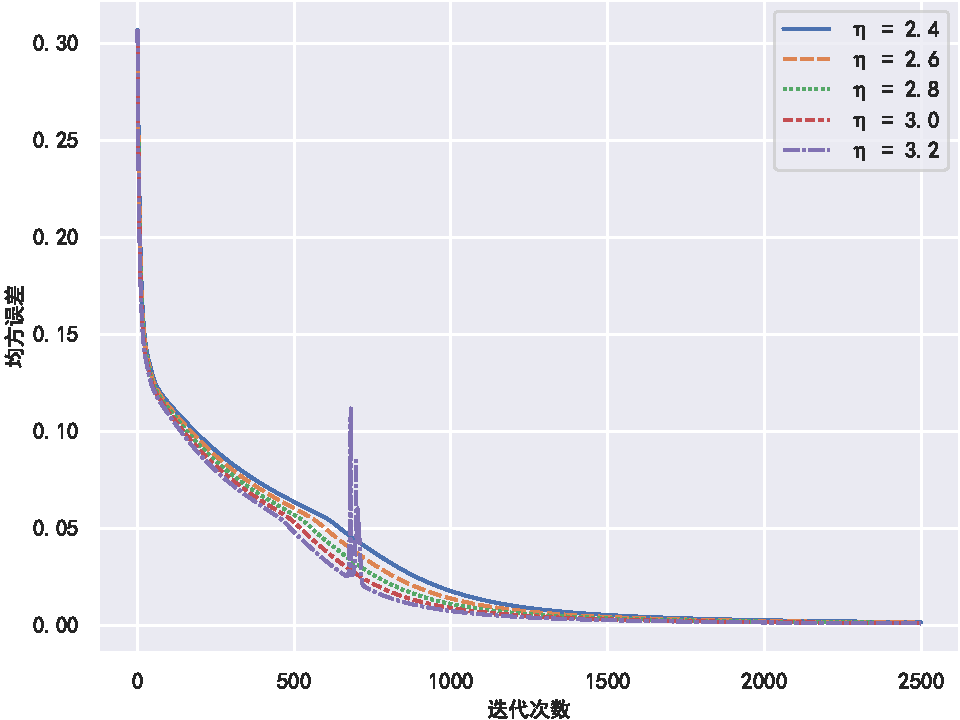
\includegraphics[width=\textwidth]{../image/累积BP抖动1.pdf}
			\caption{累积BP算法取不同$\eta$ 时的迭代速度(1)}
			\label{累积1}%文中引用该图片代号
		\end{minipage}
		\begin{minipage}{0.49\linewidth}
			\centering
			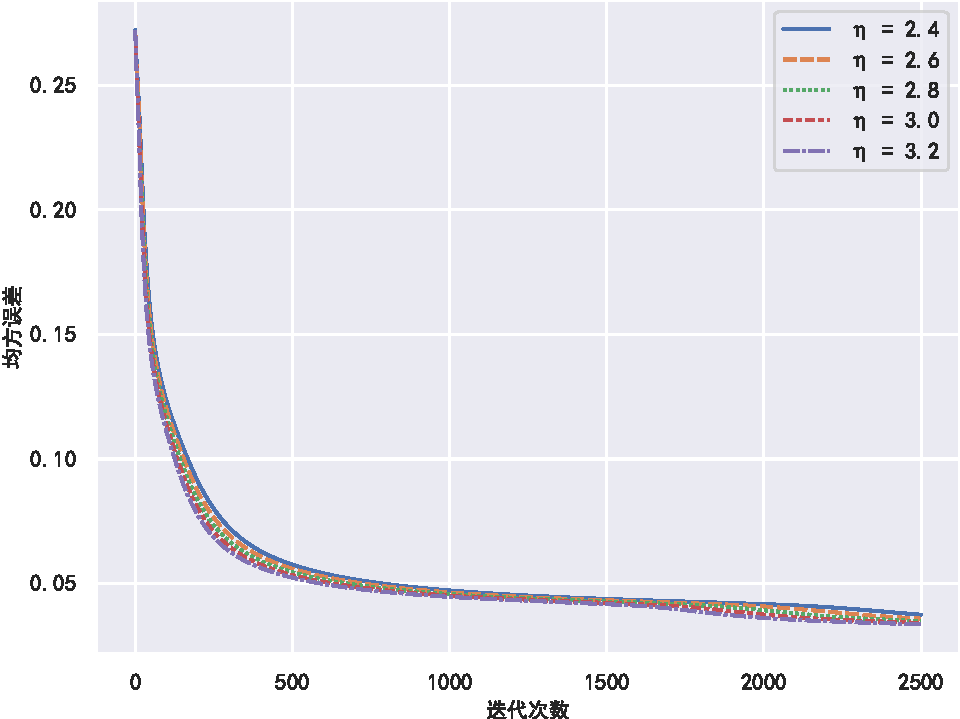
\includegraphics[width=\textwidth]{../image/累积BP抖动2.pdf}
			\caption{累积BP算法取不同$\eta$ 时的迭代速度(2)}
			\label{累积2}%文中引用该图片代号
		\end{minipage}
		%让图片换行,
		
		\begin{minipage}{0.49\linewidth}
			\centering
			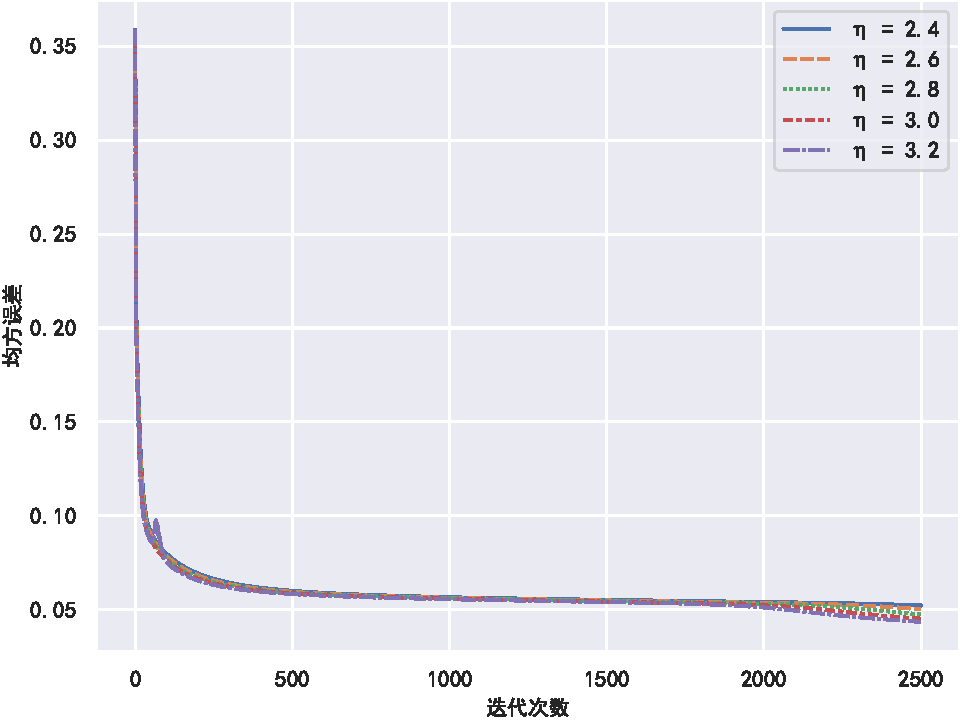
\includegraphics[width=\textwidth]{../image/累积BP抖动3.pdf}
			\caption{累积BP算法取不同$\eta$ 时的迭代速度(3)}
			\label{累积3}%文中引用该图片代号
		\end{minipage}
		\begin{minipage}{0.49\linewidth}
			\centering
			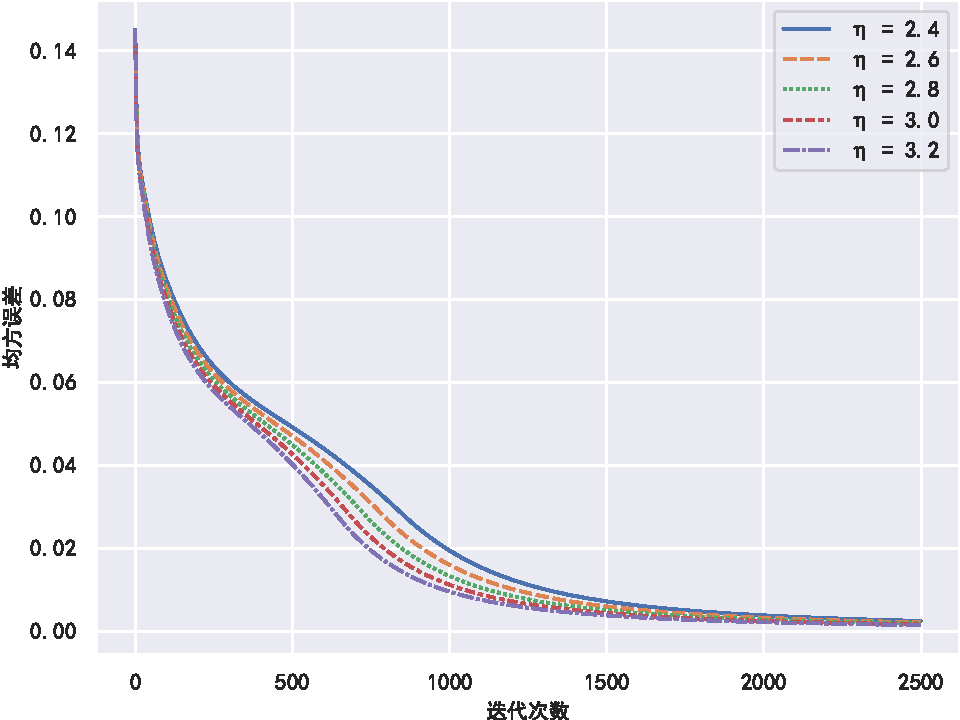
\includegraphics[width=\textwidth]{../image/累积BP抖动4.pdf}
			\caption{累积BP算法取不同$\eta$ 时的迭代速度(4)}
			\label{累积4}%文中引用该图片代号
		\end{minipage}
	\end{figure}
	
	\begin{figure}[!htb]
		\centering
		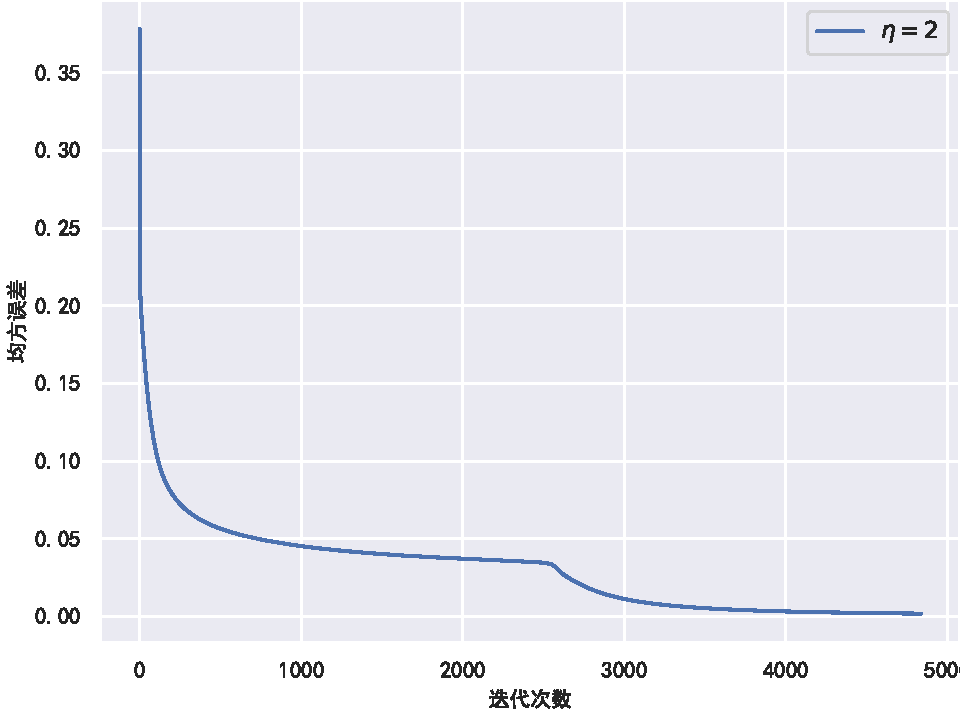
\includegraphics[height=6cm]{../image/累积BP较好值.pdf}
		\caption{累积BP算法超参数 $\eta$ 在西瓜数据集3.0上的适宜值}
		\label{累积BP适宜值}
	\end{figure}
	
	\begin{figure}[!htb]
		\centering
		\begin{minipage}{0.49\linewidth}
			\centering
			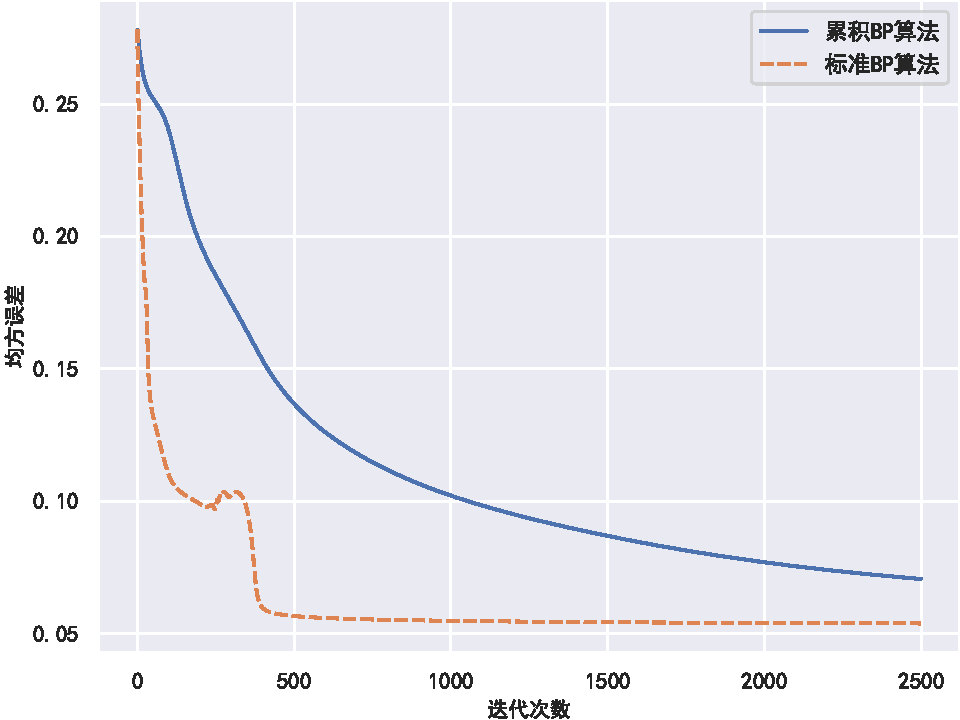
\includegraphics[width=\textwidth]{../image/比较1.pdf}
			\caption{比较标准BP算法与累积BP算法(1)}
			\label{比较1}%文中引用该图片代号
		\end{minipage}
		\begin{minipage}{0.49\linewidth}
			\centering
			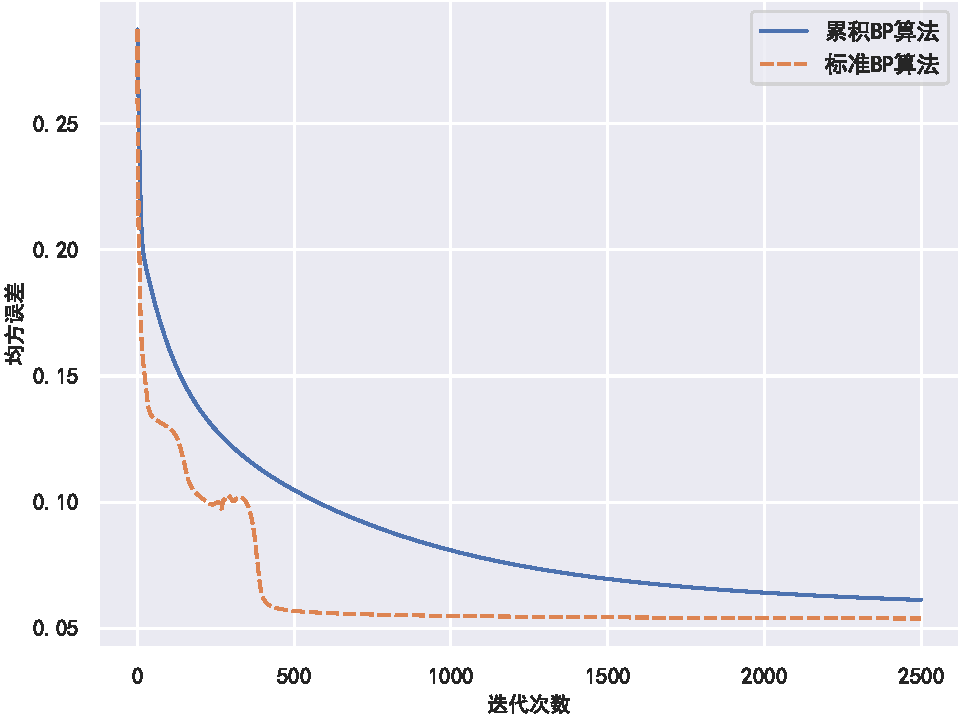
\includegraphics[width=\textwidth]{../image/比较2.pdf}
			\caption{比较标准BP算法与累积BP算法(2)}
			\label{比较2}%文中引用该图片代号
		\end{minipage}
		%让图片换行,
		
		\begin{minipage}{0.49\linewidth}
			\centering
			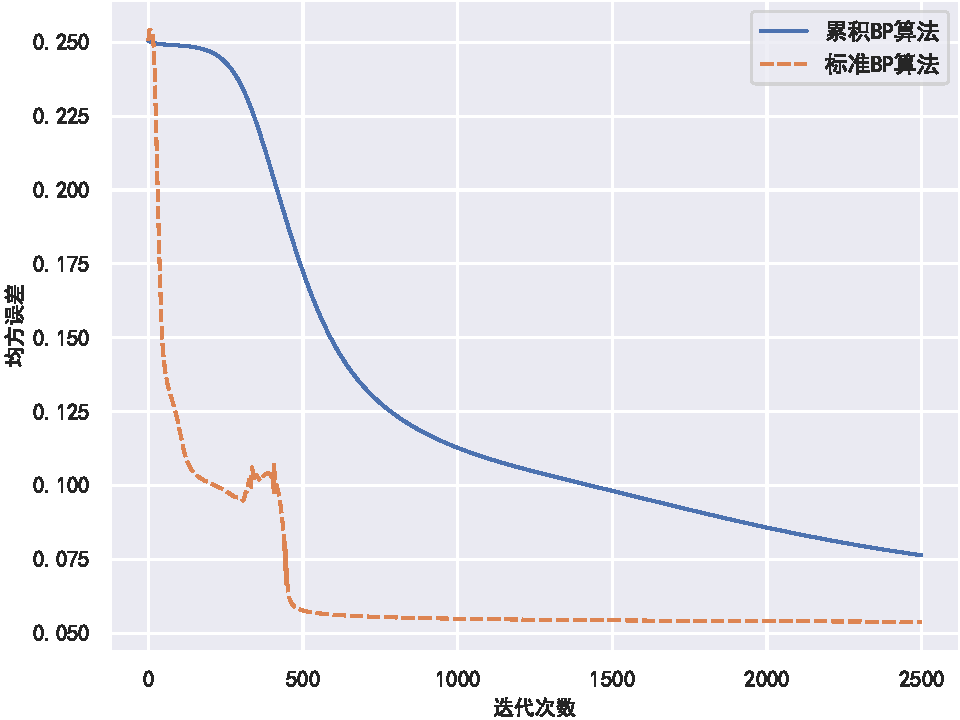
\includegraphics[width=\textwidth]{../image/比较3.pdf}
			\caption{比较标准BP算法与累积BP算法(3)}
			\label{比较3}%文中引用该图片代号
		\end{minipage}
		\begin{minipage}{0.49\linewidth}
			\centering
			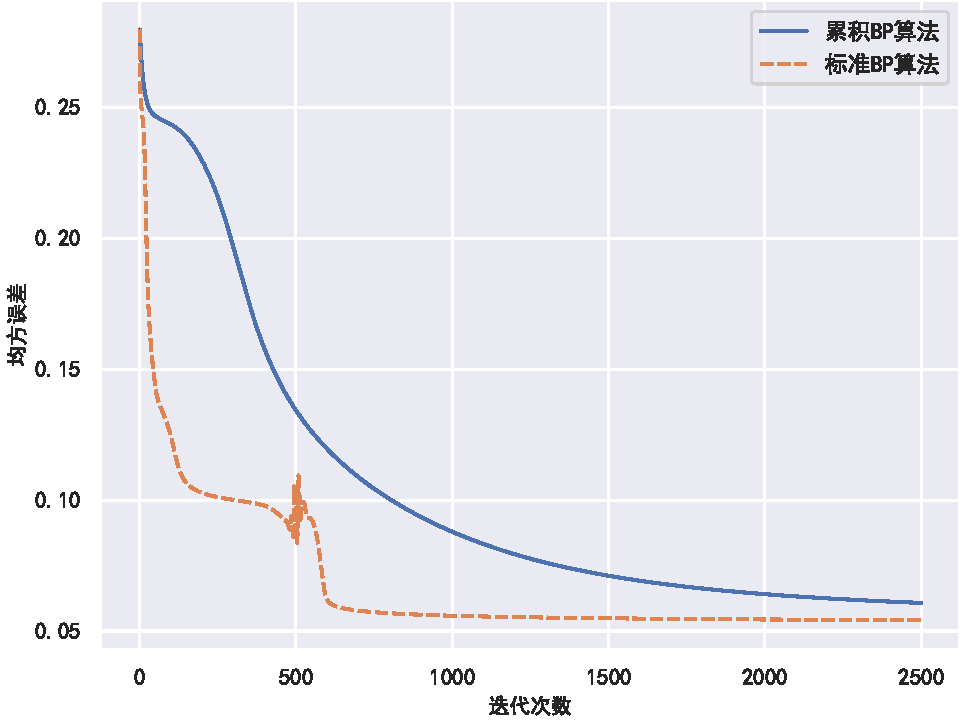
\includegraphics[width=\textwidth]{../image/比较4.pdf}
			\caption{比较标准BP算法与累积BP算法(4)}
			\label{比较4}%文中引用该图片代号
		\end{minipage}
	\end{figure}
	
	\subsection{学习收获}
	
	在此次实验中,我实现了累积BP算法,并对学习率参数 $\eta$ 进行了一些研究,得到了迭代收敛速率关于学习率的一些性质。此外,我还对标准BP算法和累积BP算法进行了比较,其差异类似于随机梯度下降与标准梯度下降之间的区别。
	
	\subsection{参考资料}
	
	\begin{itemize}
		\item 《机器学习》5.3;周志华;清华大学出版社。
	\end{itemize}
	
\end{document}